
From the discussion in the introduction, to prove Theorem~\ref{main} it is sufficient to prove the following result.

\begin{theorem}\label{Theorem_Ringel_proof}
For sufficiently large $n$, every ND-coloured $K_{2n+1}$ has a rainbow copy of every $n$-edge tree.
\end{theorem}

That is, for large $n$, and each $(n+1)$-vertex tree $T$, we seek a rainbow copy of $T$ in the ND-colouring of the complete graph with $2n+1$ vertices, $K_{2n+1}$. Our approach varies according to which of 3 cases the tree $T$ belongs to. For some small $\delta>0$, we show that, for every large $n$, every $(n+1)$-vertex tree falls in one of the following 3 cases (see Lemma~\ref{Lemma_case_division}), where a bare path is one whose internal vertices have degree 2 in the parent tree.

\begin{enumerate}[label = \Alph{enumi}]
\item $T$ has at least $\delta^6 n$ non-neighbouring leaves.
\item $T$ has at least $\delta n/800$ vertex-disjoint bare paths with length $\delta^{-1}$.
\item Removing leaves next to vertices adjacent to at least $\delta^{-4}$ leaves gives a tree with at most
$n/100$ vertices.
\end{enumerate}

As defined above, our cases are not mutually disjoint. In practice, we will only use our embeddings for trees in Case A and B which are not in Case C. In~\cite{MPS}, we developed methods to embed any $(1-\eps)n$-vertex tree in a rainbow fashion into any 2-factorized $K_{2n+1}$, where $n$ is sufficiently large depending on $\eps$. A colouring is a \emph{2-factorization} if every vertex is adjacent to exactly 2 edges of each colour. In this paper, we embed any $(n+1)$-vertex tree $T$ in a rainbow fashion into a specific 2-factorized colouring of $K_{2n+1}$, the ND-colouring, when $n$ is large. To do this, we introduce three key new methods, as follows.

\begin{enumerate}[label = {\bfseries M\arabic{enumi}}]

\item We use our results from \cite{montgomery2018decompositions} to suitably randomize the results of \cite{MPS}. This allows us to randomly embed a $(1-\eps)n$-vertex tree into any 2-factorized $K_{2n+1}$, so that the image is rainbow and has certain random properties. These properties allow us to apply a case-appropriate \emph{finishing lemma} with the uncovered colours and vertices.\label{T2}
\item We use a new implementation of absorption to embed a small part of $T$ while using some vertices in a random subset of $V(K_{2n+1})$ and exactly the colours in a random subset of $C(K_{2n+1})$. This uses different \emph{absorption structures} for trees in Case A and in Case B, and in each case gives the finishing lemma for that case.\label{T1}
\item We use an entirely new, deterministic, embedding for trees in Case C.\label{T3}
\end{enumerate}

 For trees in Cases A and B, we start by finding a random rainbow copy of most of the tree using~\ref{T2}, as outlined in Section~\ref{sec:T2}. Then, we embed the rest of the tree using uncovered vertices and exactly the unused colours using~\ref{T1}, which gives a finishing lemma for each case. These finishing lemmas are discussed in Section~\ref{sec:T1}. We use \ref{T3} to embed trees in Case C, which is essentially independent of our embeddings of trees in Cases A and B. This method is outlined in Section \ref{sec:T3}. In Section~\ref{sec:overhead}, we state our main lemmas and theorems, and prove Theorem~\ref{Theorem_Ringel_proof} subject to these results.

The rest of the paper is structured as follows. Following details of our notation, in Section~\ref{sec:prelim} we recall and prove various preliminary results.  We then prove the finishing lemma for Case A in Section~\ref{sec:finishA} and the finishing lemma for Case B in Section~\ref{sec:finishB} (together giving \ref{T1}). In Section~\ref{sec:almost}, we give our randomized rainbow embedding of most of the tree (\ref{T2}). In Section~\ref{sec:lastC}, we embed the trees in Case C with a deterministic embedding (\ref{T3}). Finally, in Section~\ref{sec:conc}, we make some concluding remarks.


\subsection{\ref{T2}: Embedding almost all of the tree randomly in Cases A and B}\label{sec:T2}
For a tree $T$ in Case A or B, we carefully choose a large subforest, $T'$ say, of $T$, which contains almost all the edges of $T$. We find a rainbow copy $\hat{T}'$ of $T'$ in the ND-colouring of $K_{2n+1}$ (which exists due to~\cite{MPS}), before applying a finishing lemma to extend $\hat{T}'$ to a rainbow copy of $T$. Extending to a rainbow copy of $T$ is a delicate business --- we must use exactly the $n-e(\hat{T})$ unused colours. Not every rainbow copy of $T'$ will be extendable to a rainbow copy of $T$. However, by combining our methods in \cite{montgomery2018decompositions} and \cite{MPS}, we can take a random rainbow copy $\hat{T}'$ of $T'$ and show that it is likely to be extendable to a rainbow copy of $T$. Therefore, some rainbow copy of $T$ must exist in the ND-colouring of $K_{2n+1}$.

As $\hat{T}'$ is random, the sets $\bar{V}:=V(K_{2n+1})\setminus V(\hat{T})$ and $\bar{C}:=C(K_{2n+1})\setminus C(\hat{T})$ will also be random.  The distributions of $\bar{V}$ and $\bar{C}$ will be complicated, but we will not need to know them. It will suffice that there will be large (random) subsets $V\subset \bar{V}$ and $C\subset \bar{C}$ which each do have a nice, known, distribution.
Here, for example, $V\subset V(K_{2n+1})$ has a nice distribution if there is some $q$ so that each element of $V(K_{2n+1})$ appears independently at random in $V$ with probability $q$ --- we say here that $V$ is \emph{$q$-random} if so, and analogously we define a $q$-random subset $C\subset C(K_{2n+1})$ (see Section~\ref{sec:prob}). A natural combination of the techniques in~\cite{montgomery2018decompositions,MPS} gives the following.
\begin{theorem}\label{Sketch_Near_Embedding} For each $\epsilon>0$, the following holds for sufficiently large $n$.
Let $K_{2n+1}$ be $2$-factorized and let $T'$ be a forest on $(1-\epsilon)n$ vertices. Then, there is a randomized subgraph $\hat{T}'$ of $K_{2n+1}$ and random subsets $V\subset V(K_{2n+1})\setminus V(\hat{T}')$ and $C\subset C(K_{2n+1})\setminus C(\hat{T}')$ such that the following hold for some $p:=p(T')$ (defined precisely in Theorem~\ref{nearembedagain}).
\stepcounter{propcounter}
\begin{enumerate}[label = {\bfseries \Alph{propcounter}\arabic{enumi}}]
\item $\hat{T}'$ is a rainbow copy of $T'$ with high probability.\label{woo1}
\item $V$ is $(p+\eps)/6$-random and $C$ is $(1-\epsilon)\eps$-random. ($V$ and $C$ may depend on each other.)\label{woo2}
\end{enumerate}
\end{theorem}

We will apply a variant of Theorem~\ref{Sketch_Near_Embedding} (see Theorem~\ref{nearembedagain}) to subforests of trees in Cases A and B, and there we will have that $p\gg \eps$. Note that, then, $C$ will likely be much smaller than $V$. This reflects that $\hat{T}'\subset K_{2n+1}$ will contain fewer than $n$ out of $2n+1$ vertices, while $C(K_{2n+1})\setminus C(\hat{T}')$ contains exactly $n-e(\hat{T}')$ out of $n$ colours.

As explained in~\cite{MPS}, in general the sets $V$ and $C$ cannot be independent, and this is in fact why we need to treat trees in Case C separately. In order to finish the embedding in Cases A and B, we need, essentially, to find \emph{some} independence between the sets $V$ and $C$ (as discussed below). The embedding is then as follows for some small $\delta$ governing the case division, with $\eps=\delta^6$ in Case A and $\bar{\eps}\oldgg \delta$ in Case B. Given an $(n+1)$-vertex tree $T$ in Case A or B we delete either $\epsilon n$ non-neighbouring leaves (Case A) or $\bar{\epsilon} n/k$ vertex-disjoint bare paths with length $k=\delta^{-1}$ (Case B) to obtain a forest $T'$. Using (a variant of) Theorem~\ref{Sketch_Near_Embedding}, we find a randomized rainbow copy $\hat{T}'$ of $T'$ along with some random vertex and colour sets and apply a finishing lemma to extend this to a rainbow copy of $T$.

After a quick note on the methods in~\cite{montgomery2018decompositions} and~\cite{MPS}, we will discuss the finishing lemmas, and explain why we need some independence, and how much independence is needed.


\subsubsection*{Randomly embedding nearly-spanning trees}
In~\cite{MPS}, we embedded a $(1-\epsilon)n$-vertex tree $T$ into a 2-factorization of $K_{2n+1}$ by breaking it down mostly into large stars and large matchings. For each of these, we embedded the star or matching using its own random set of vertices and random set of colours (which were not necessarily independent of each other). In doing so, we used almost all of the colours in the random colour set, but only slightly less than one half of the vertices in the random vertex set. (This worked as we had more than twice as many vertices in $K_{2n+1}$ than in $T$.)  For trees not in Case C, a substantial portion of a large subtree was broken down into matchings. By embedding these matchings more efficiently, using results from~\cite{montgomery2018decompositions}, we can use a smaller random vertex set. This reduction allows us to have, disjointly from the embedded tree, a large random vertex subset $V$.

More precisely, where $q,\epsilon\oldgg n^{-1}$, using a random set $V$ of $2qn$ vertices and a random set $C$ of $qn$ colours, in~\cite{MPS} we showed that, with high probability, from any set $X\subset V(K_{2n+1})\setminus V$ with $|X|\leq (1-\epsilon)qn$, there was a $C$-rainbow matching from $X$ into $V$. Dividing $V$ randomly into two sets $V_1$ and $V_2$, each with $qn$ vertices, and using the results in~\cite{montgomery2018decompositions}, we can use $V_1$ to find the $C$-rainbow matching (see Lemma~\ref{Lemma_MPS_nearly_perfect_matching}).
Thus, we gain the random set $V_2$ of $qn$ vertices which we do not use for the embedding of $T$, and we can instead use it to extend this to an $(n+1)$-vertex tree in $K_{2n+1}$.
Roughly speaking, if in total $pn$ vertices of $T$ are embedded using matchings, then we gain altogether a random set of around $pn$ vertices.

If a tree is not in Case C, then the subtree/subforest we embed using these techniques has plenty of vertices embedded using matchings, so that in this case we will be able to take $p\geq 10^{-3}$ when we apply the full version of Theorem~\ref{Sketch_Near_Embedding} (see Theorem~\ref{nearembedagain}). Therefore, we will have many spare vertices when adding the remaining $\eps n$ vertices to the copy of $T$. Our challenges are firstly that we need to use exactly all the colours not used on the copy of $T'$ and secondly that there can be a lot of dependence between the sets $V$ and $C$. We first discuss how we ensure that we use every colour.



\subsection{\ref{T1}: Finishing the embedding in Cases A and B}\label{sec:T1}

To find trees using every colour in an ND-coloured $K_{2n+1}$ we prove two \emph{finishing lemmas} (Lemma~\ref{lem:finishA} and~\ref{lem:finishB}).  These lemmas say that, for a given randomized set of vertices $V$ and a given randomized set of colours $C$, we can find a rainbow matching/path-forest which uses exactly the colours in $C$, while using some of the vertices from $V$.  These lemmas are used to finish the embedding of the trees in Cases A and B, where the last step is to (respectively) embed a matching or path-forest that we removed from the tree $T$ to get the forest $T'$. Applying (a version of) Theorem~\ref{Sketch_Near_Embedding} we get a random rainbow copy $\hat{T'}$ of $T'$ and random sets $\bar{V}=V(K_n)\setminus V(\hat{T}')$ and $\bar{C}=C(K_n)\setminus C(\hat{T}')$.

In order to apply the case-appropriate finishing lemma, we need some independence between $\bar{V}$ and $\bar{C}$, for reasons we now discuss for Case A, and then Case B. Next, we discuss the independence property we use and how we achieve this independence. (Essentially, this property is that $\bar{V}$ and $\bar{C}$ contain two small random subsets which are independent of each other.) Finally, we discuss the absorption ideas for Case A and Case B.




\subsubsection*{Finishing with matchings (for Case A)}
In Case A, we take the $(n+1)$-vertex tree $T$ and remove a large matching of leaves, $M$ say, to get a tree, $T'$ say, that can be embedded using Theorem~\ref{Sketch_Near_Embedding}. This gives a random copy, $\hat{T}'$ say, of $T'$ along with random sets $V\subset V(K_{2n+1})\setminus V(\hat{T}')$ and $C\subset C(K_{2n+1})\setminus C(\hat{T}')$
 which are $(p+\eps)/6$-random and $(1-\eps)\eps$-random respectively. For trees not in Case C we will have $p\oldgg \eps$.
 Let $X\subset V(\hat{T}')$ be the set of vertices we need to add neighbours to as leaves to make $\hat{T}'$ into a copy of $T$.

We would like to find a perfect matching from $X$ to $\bar{V}:=V(K_{2n+1})\setminus V(\hat{T}')$ with exactly the colours in $\bar{C}:=C(K_{2n+1})\setminus C(\hat{T}')$, using that $V\subset \bar{V}$ and $C\subset \bar{C}$. (A perfect matching from $X$ to $\bar{V}$ is such a matching covering every vertex in $X$.)
 Unfortunately, there may be some $x\in X$ with no edges with colour in $\bar{C}$ leading to $\bar{V}$. (If $C$ and $V$ were independent, then this would not happen with high probability.) If this happens, then the desired matching will not exist.

In Case B, a very similar situation to this may occur, as discussed below, but in Case A there is another potential problem. There may be some colour $c\in \bar{C}$ which does not appear between $X$ and $\bar{V}$, again preventing the desired matching existing. This we will avoid by carefully embedding a small part of $T'$ so that every colour appears between $X$ and $\bar{V}$ on plenty of edges.



\subsubsection*{Finishing with paths (for Case B)}
In Case B, we take the $(n+1)$-vertex tree $T$ and remove a set of vertex-disjoint bare paths to get a forest, $T'$ say, that can be embedded using Theorem~\ref{Sketch_Near_Embedding}. This gives a random copy, $\hat{T}'$ say, of $T'$ along with random sets $V\subset V(K_{2n+1})\setminus V(\hat{T}')$ and $C\subset C(K_{2n+1})\setminus C(\hat{T}')$
 which are $(p+\eps)/6$-random and $(1-\eps)\eps$-random respectively. For trees not in Case C we will have $p\oldgg \eps$.

 Let $\ell$ and $X=\{x_1,\ldots,x_\ell,y_1,\ldots,y_\ell\}\subset V(\hat{T}')$ be such that to get a copy of $T$ from $\hat{T}'$ we need to add vertex-disjointly a suitable path between $x_i$ and $y_i$, for each $i\in [\ell]$.
We would like to find these paths with interior vertices in $\bar{V}:= V(K_{2n+1})\setminus V(\hat{T}')$ so that their edges are collectively rainbow with exactly the colours in $\bar{C}:=C(K_{2n+1})\setminus C(\hat{T}')$, using that $V\subset \bar{V}$ $C\subset \bar{C}$. Unfortunately, there may be some $x\in X$ with no edges with colour in $\bar{C}$ leading to $V$. (If $C$ and $V$ were independent, then, again, this would not happen with high probability.) If this happens, then the desired paths will not exist.

Note that the analogous version of the second problem in Case A does not arise in Case B. Here,  it is likely that every colour appears on many edges within $V$, so that we can use any colour by putting an appropriate edge within $V$ in the middle of one of the missing paths.

\subsubsection*{Retaining some independence}
To avoid the problem common to Cases A and B, when proving our version of Theorem~\ref{Sketch_Near_Embedding} (that is, Theorem~\ref{nearembedagain}), we set aside small random sets $V_0$ and $C_0$ early in the embedding, before the dependence between colours and vertices arises. This gives us a version of Theorem~\ref{Sketch_Near_Embedding} with the additional property that, for some $\mu\oldll \eps$, there are additional random sets $V_0\subset V(K_{2n+1})\setminus (V(\hat{T}')\cup V)$ and $C_0\subset C(K_{2n+1})\setminus (C(\hat{T}')\cup C)$ such that the following holds in addition to \ref{woo1} and \ref{woo2}.

\begin{enumerate}[label = {\bfseries \Alph{propcounter}\arabic{enumi}}]\addtocounter{enumi}{2}
\item $V_0$ is a $\mu$-random subset of $V(K_{2n+1})$, $C_0$ is a $\mu$-random subset of $C(K_{2n+1})$, and they are independent of each other.\label{propq2}
\end{enumerate}

\noindent
Then, by this independence, with high probability, every vertex in $K_{2n+1}$ will have $\mu^2 n/2$ adjacent edges with colour in $C_0$ going into the set $V_0$ (see Lemma~\ref{Lemma_high_degree_into_random_set}).

To avoid the problem that only arises in Case A, consider the set $U\subset V(T')$ of vertices which need leaves added to them to reach $T$ from $T'$. By carefully embedding a small subtree of $T'$ containing plenty of vertices in $U$, we ensure that, with high probability, each colour appears plenty of times between the image of $U$ and $V_0$. That is, we have the following additional property for some $1/n\oldll \xi\oldll \mu$.

\begin{enumerate}[label = {\bfseries \Alph{propcounter}\arabic{enumi}}]\addtocounter{enumi}{3}
\item With high probability, if $Z$ is the copy of $U$ in $\hat{T}'$, then every colour in  $C(K_{2n+1})$, has at least $\xi n$ edges between $Z$ and $V_0$.\label{propq1}
\end{enumerate}

Of course, \ref{propq2} and \ref{propq1} do not show that our desired matching/path-collection exists, only that (with high probability) there is no single colour or vertex preventing its existence. To move from this to find the actual matching/path-collection we use \emph{distributive absorption}.



\subsubsection*{Distributive absorption}
To prove our finishing lemmas, we use an \emph{absorption strategy}. Absorption has its origins in work by Erd\H{o}s, Gy\'arf\'as and Pyber~\cite{EP} and Krivelevich~\cite{MKtri}, but was codified  by R\"odl, Ruci\'nski and Szemer\'edi~\cite{RRS} as a versatile technique
for extending approximate results into exact ones. For both Case A and Case B we use a new implementation of \emph{distributive absorption}, a method introduced by the first author in~\cite{montgomery2018spanning}.

To describe our absorption, let us concentrate on Case A. Our methods in Case B are closely related, and we comment on these afterwards. To recap, we have a random rainbow tree $\hat{T}'$ in the ND-colouring of  $K_{2n+1}$ and a set $X\subset V(\hat{T})$, so that we need to add a perfect matching from  $X$ into $\bar{V}=V(K_{2n+1})\setminus V(\hat{T}')$ to make $\hat{T}'$ into a copy of $T$. We wish to add this matching in a rainbow fashion using (exactly) the colours in $\bar{C}= C(K_{2n+1})\setminus C(\hat{T})$.

To use distributive absorption, we first show that for any set $\hat{C}\subset C(K_{2n+1})$ of at most 100 colours, we can find a set $D\subset \bar{C}\setminus C$ and sets $X'\subset X$ and $V'\subset \bar{V}$ with $|D|\leq 10^3$, $|V'|\leq 10^4$ and $|X'|=|D|+1$, so that the following holds.
\stepcounter{propcounter}
\begin{enumerate}[label = {\bfseries \Alph{propcounter}\arabic{enumi}}]
    \item Given any colour $c\in\hat{C}$, there is a perfect $(D\cup \{c\})$-rainbow matching from $X'$ to $V'$.\label{switchprop}
\end{enumerate} 

We call such a triple $(D,X',V')$ a \emph{switcher} for $\hat{C}$. AS $|\bar{C}|=|X|$, a perfect $(\bar{C}\setminus D)$-rainbow matching from $X\setminus X'$ into $V\setminus V'$ uses all but 1 colour in $\bar{C}\setminus D$. If we can find such a matching whose unused colour, $c$ say, lies in $\hat{C}$, then using \ref{switchprop}, we can find a perfect $(D\cup\{c\})$-rainbow matching from $X'$ to $V'$. Then, the two matchings combined form a perfect $\bar{C}$-rainbow matching from $X$ into $V$, as required.

The switcher outlined above only gives us a tiny local variability property, reducing finding a large perfect matching with exactly the right number of colours to finding a large perfect matching with one spare colour so that the unused colour lies in a small set (the set $\bar{C}$). However, by finding many switchers for carefully chosen sets $\hat{C}$, we can build this into a global variability property. These switchers can be found using different vertices and colours (see Section~\ref{sec:switcherspaths}), so that matchings found using the respective properties \ref{switchprop} can be combined in our embedding. 

We choose different sets $\hat{C}$ for which to find a switcher by using an auxillary graph as a template. This template is a \emph{robustly matchable bipartite graph} --- a bipartite graph, $K$ say, with vertex classes $U$ and $Y\cup Z$ (where $Y$ and $Z$ are disjoint), with the following property.

\begin{enumerate}[label = {\bfseries \Alph{propcounter}\arabic{enumi}}]\addtocounter{enumi}{1}
\item For any set $Z^\ast\subset Z$ with size $|U|-|Y|$, there is a perfect matching in $K$ between $U$ and $Y\cup Z^\ast$.
\end{enumerate}

Such bipartite graphs were shown to exist by the first author~\cite{montgomery2018spanning}, and, furthermore, for large $m$ and $\ell\leq m$, we can find such a graph with maximum degree at most 100, $|U|=3m$, $|Y|=2m$ and $|Z|=m+\ell$ (see Lemma~\ref{Lemma_H_graph}). 
To use the template, we take disjoint sets of colours, $C'=\{c_v:v\in Y\}$ and $C''=\{c_v:v\in Z\}$ in $\bar{C}$. For each $u\in U$, we find a switcher $(D_u,X_u,V_u)$ for the set of colours $\{c_v:v\in N_K(u)\}$. Furthermore, we do this so that the sets $D_u$ are disjoint and in $\bar{C}\setminus (C'\cup C'')$, and the sets $X_u$, and $V_u$, are disjoint and in $X$, and $\bar{V}$, respectively.  We can then show we have the following property.
\begin{enumerate}[label = {\bfseries \Alph{propcounter}\arabic{enumi}}]\addtocounter{enumi}{2}
\item For any set $C^*\subset C''$ of $m$ colours, there is a perfect $(C^*\cup C'\cup(\cup_{u\in U}D_u))$-rainbow matching from $\cup_{u\in U}X_u$ into $\cup_{u\in U}V_u$.\label{Kprop}
\end{enumerate}
Indeed, to see this, take any set of $C^*\subset C''$ of $m$ colours, let $Z^*=\{v:c_v\in C^*\}$ and note that $|Z^*|=m$. By \ref{Kprop}, there is a perfect matching in $K$ from $U$ into $Y\cup Z^\ast$, corresponding to the function $f:U\to Y\cup Z^*$ say. For each $u\in U$, using that $(D_u,X_u,V_u)$ is a switcher for $\{c_v:v\in N_K(u)\}$ and $uf(u)\in E(K)$, find a perfect $(D_u\cup \{c_{f(u)}\})$-rainbow matching $M_u$ from $X_u$ to $V_u$.
As the sets $D_u$, $X_u$, $V_u$, $u\in U$, are disjoint, $\cup_{u\in U}M_u$ is a perfect $(C^*\cup C'\cup(\cup_{u\in U}D_u))$-rainbow matching from $\cup_{u\in U}X_u$ into $\cup_{u\in U}V_u$, as required.

Thus, we have a set of colours $C''$ from which we are free to use any $\ell$ colours, and then use the remaining colours together with $C'\cup(\cup_{u\in U}D_u)$ to find a perfect rainbow matching from $\cup_{u\in U}X_u$ into $\cup_{u\in U}V_u$. By letting $m$ be as large as allowed by our construction methods, and $C''$ be a random set of colours, we have a useful \emph{reservoir} of colours, so that we can find a structure in $T$ using $\ell$ colours in $C''$, and then finish by attaching a matching to $\cup_{u\in U}X_u$.


%We say that we \emph{absorb} the $m$ unused colours in $C$ to find, along with the colours in $C'\cup(\cup_{u\in U}D_u)$ and vertices $\cup_{u\in U}V_u$, the matching from $\cup_{u\in U}X_u$.

We have two things to consider to fit this final step into our proof structure, which we discuss below. Firstly, we can only absorb colours in $C''$, so after we have covered most of the colours, we need to cover the unused colours outside of $C''$ (essentially achieved by \ref{propp2} below). Secondly, we find the switchers greedily in a random set. There are many more unused colours from this set than we can absorb, and the unused colours no longer have good random properties, so we also need to reduce the unused colours to a number that we can absorb (essentially achieved by \ref{propp1} below).


\subsubsection*{Creating our finishing lemmas using absorption}
To recap, we wish to find a perfect $\bar{C}$-rainbow matching from $X$ into $\bar{V}$. To do this, it is sufficient to find partitions $X=X_1\cup X_2\cup X_3$, $\bar{V}=V_1\cup V_2\cup V_3$ and $\bar{C}=C_1\cup C_2\cup C_3$ with the following properties.
\stepcounter{propcounter}
\begin{enumerate}[label = {\bfseries \Alph{propcounter}\arabic{enumi}}]
\item There is a perfect $C_1$-rainbow matching from $X_1$ into $V_1$. \label{propp1}
\item Given any set of colours $C'\subset C_1$ with $|C'|\leq |C_1|-|X_1|$, there is a perfect $(C_2\cup C')$-rainbow matching from $X_2$ into $V_2$ which uses each colour in $C'$.\label{propp2}
\item Given any set of colours $C''\subset C_2$ with size $|X_3|-|C_3|$, there is a perfect  $(C''\cup C_3)$-rainbow matching from $X_3$ into $V_3$.\label{propp3}
\end{enumerate}
Finding such a partition requires the combination of all our methods for Case A. In brief, however, we develop \ref{propp1} using a result from~\cite{montgomery2018decompositions} (see Lemma~\ref{Lemma_MPS_nearly_perfect_matching}), we develop \ref{propp2} using the condition \ref{propq1}, and we develop \ref{propp3} using the distributive absorption strategy outlined above.

If we can find such a partition, then we can easily show that the matching we want must exist. Indeed, given such a partition, then, using \ref{propp1}, let $M_1$ be a perfect $C_1$-rainbow matching from $X_1$ into $V_1$, and let $C'=C_1\setminus C(M_1)$. Using~\ref{propp2}, let $M_2$ be a perfect  $(C_2\cup C')$-rainbow matching from $X_2$ into $V_2$ which uses each colour in $C'$, and let $C''=(C_2\cup C')\setminus C(M)=C_2\setminus C(M)$. Finally, noting that $|C''|+|C_3|=|\bar{C}|-|X_1|-|X_2|=|X_3|$, using~\ref{propp3}, let $M_3$ be a perfect $(C''\cup C_3)$-rainbow matching from $X_3$ into $V_3$. Then, $M_1\cup M_2\cup M_3$ is a $\bar{C}$-rainbow matching from $X$ into $\bar{V}$.


The above outline also lies behind our embedding in Case B, where we finish instead by embedding $\ell$ paths vertex-disjointly between certain vertex pairs, for some $\ell$. Instead of the partition $X_1\cup X_2\cup X_3$ we have a partition $[\ell]=I_1\cup I_2\cup I_3$, and, instead of each matching from $X_i$ to $V_i$, $i\in [3]$, we find a set of vertex-disjoint $x_j,y_j$-paths, $j\in I_i$, with interior vertices in $V_i$ which are collectively $C_i$-rainbow. The main difference is how we construct switchers using paths instead of matchings (see Section~\ref{sec:switchers}).






\subsection{\ref{T3}: The embedding in Case C}\label{sec:T3}
After large clusters of adjacent leaves are removed from a tree in Case C, few vertices remain. We remove these large clusters, from the tree, $T$ say, to get the tree $T'$, and carefully embed $T'$ into the ND-colouring using a deterministic embedding. The image of this deterministic embedding occupies a small interval in the ordering used to create the ND-colouring. Furthermore, the embedded vertices of $T'$ which need leaves added to create a copy of $T$ are well-distributed within this interval. These properties will allow us to embed the missing leaves using the remaining colours. This is given more precisely in Section~\ref{sec:caseC}, but in order to illustrate this in the easiest case, we will give the embedding when there is exactly one vertex with high degree.


Our embedding in this case is rather simple. Removing the leaves incident to a very high degree vertex, we embed the rest of the tree into $[n]$ so that the high degree vertex is embedded to 1. The missing leaves are then embedded into $[2n+1]\setminus [n]$ using the unused colours.

\begin{theorem}[One large vertex]\label{Theorem_one_large_vertex}
Let $n\geq 10^6$. Let $K_{2n+1}$ be $ND$-coloured, and let $T$ be an $(n+1)$-vertex tree containing a vertex $v_1$ which is adjacent to $\geq 2n/3$ leaves.
Then, $K_{2n+1}$ contains a rainbow copy of $T$.
\end{theorem}
\begin{proof}
See Figure~\ref{Figure_1_vertex} for an illustration of this proof.
Let $T'$ be $T$ with the neighbours of $v_1$ removed and let $m=|T'|$. By assumption, $|T'|\leq n/3+1$. Order the vertices of $T'-v_1$ as $v_2, \dots, v_{m}$ so that $T[v_1, \dots, v_i]$ is a tree for each $i\in [m]$. Embed $v_1$ to $1$ in $K_{2n+1}$, and then greedily embed $v_2, \dots, v_m$ in turn to some vertex in $[n]$ so that the copy
of $T'$ which is formed is rainbow in $K_{2n+1}$. This is possible since at each step at most $|T'|\leq n/3$ of the vertices in $[n]$ are occupied, and at most $e(T')\leq n/3-1$ colours are used. Since the $ND$-colouring has 2 edges of each colour adjacent to each vertex,
this forbids at most $n/3+2(n/3-1)=n-2$ vertices in $[n]$. Thus, we can embed each $v_{i}$, $2\leq i\leq m$ using an unoccupied vertex in $[n]$ so that the edge from $v_i$ to $v_1, \ldots, v_{i-1}$ has a colour that we have not yet used. Let $S'$ be the resulting rainbow copy of $T'$, so that $V(S')\subset [n]$.

Let $S$ be $S'$ together with the edges between $1$ and $2n+2-c$ for every $c\in [n]\setminus C(S')$. Note that the neighbours added are all bigger than $n$, and so the resulting graph is a tree. There are exactly $n-e(T')$ edges added, so $S$ is a copy of $T$. Finally, for each $c\in [n]\setminus C(S')$, the edge from $1$ to $2n+2-c$ is colour $c$, so the resulting tree is rainbow.
\end{proof}

\begin{figure}[h]

\vspace{-0.1cm}

\begin{center}
{

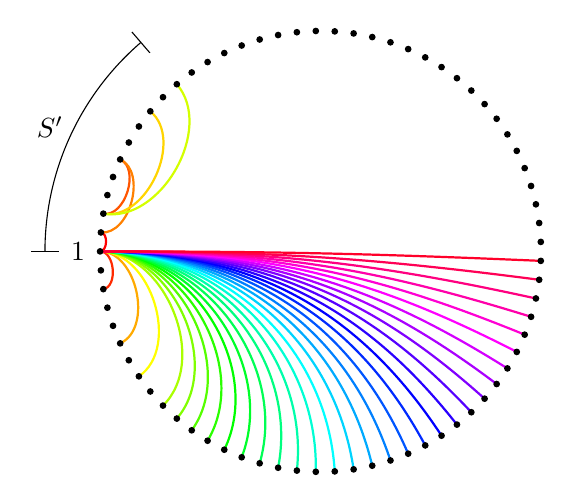
\begin{tikzpicture}[scale=0.7,define rgb/.code={\definecolor{mycolor}{rgb}{#1}},
                    rgb color/.style={define rgb={#1},mycolor},reflect at xaxis/.style={xshift=1cm,xscale=-1,xshift=-1*1cm}]


%\foreach \x in {1,...,36}
%{
%\draw [rgb color={1,0,0}] (0:4) to [in={4.9315068493*\x+180},out={0+180}] ({4.9315068493
%*\x}:4);
%}


\begin{scope}[reflect at xaxis,rotate=0]

\draw [thick,rgb color={1,0,0}, rotate = -4.9315068493*0] (0:4) to [in={4.9315068493*1+180},out=180] ({4.9315068493 *1}:4);
\draw [thick,rgb color={1,0.166666666666667,0}, rotate = -4.9315068493*2] (0:4) to [in={4.9315068493*2+180},out=180] ({4.9315068493 *2}:4);
\draw [thick,rgb color={1,0.333333333333333,0}, rotate = 4.9315068493*2] (0:4) to [in={4.9315068493*3+180},out=180] ({4.9315068493 *3}:4);
\draw [thick,rgb color={1,0.5,0}, rotate = 4.9315068493*1] (0:4) to [in={4.9315068493*4+180},out=180] ({4.9315068493 *4}:4);
\draw [thick,rgb color={1,0.666666666666667,0}, rotate = -4.9315068493*5] (0:4) to [in={4.9315068493*5+180},out=180] ({4.9315068493 *5}:4);
\draw [thick,rgb color={1,0.833333333333333,0}, rotate = 4.9315068493*2] (0:4) to [in={4.9315068493*6+180},out=180] ({4.9315068493 *6}:4);
\draw [thick,rgb color={1,1,0}, rotate = -4.9315068493*7] (0:4) to [in={4.9315068493*7+180},out=180] ({4.9315068493 *7}:4);
\draw [thick,rgb color={0.833333333333333,1,0}, rotate = 4.9315068493*2] (0:4) to [in={4.9315068493*8+180},out=180] ({4.9315068493 *8}:4);
\draw [thick,rgb color={0.666666666666667,1,0}, rotate = -4.9315068493*9] (0:4) to [in={4.9315068493*9+180},out=180] ({4.9315068493 *9}:4);
\draw [thick,rgb color={0.5,1,0}, rotate = -4.9315068493*10] (0:4) to [in={4.9315068493*10+180},out=180] ({4.9315068493 *10}:4);
\draw [thick,rgb color={0.333333333333333,1,0}, rotate = -4.9315068493*11] (0:4) to [in={4.9315068493*11+180},out=180] ({4.9315068493 *11}:4);
\draw [thick,rgb color={0.166666666666667,1,0}, rotate = -4.9315068493*12] (0:4) to [in={4.9315068493*12+180},out=180] ({4.9315068493 *12}:4);
\draw [thick,rgb color={0,1,0}, rotate = -4.9315068493*13] (0:4) to [in={4.9315068493*13+180},out=180] ({4.9315068493 *13}:4);
\draw [thick,rgb color={0,1,0.166666666666667}, rotate = -4.9315068493*14] (0:4) to [in={4.9315068493*14+180},out=180] ({4.9315068493 *14}:4);
\draw [thick,rgb color={0,1,0.333333333333333}, rotate = -4.9315068493*15] (0:4) to [in={4.9315068493*15+180},out=180] ({4.9315068493 *15}:4);
\draw [thick,rgb color={0,1,0.5}, rotate = -4.9315068493*16] (0:4) to [in={4.9315068493*16+180},out=180] ({4.9315068493 *16}:4);
\draw [thick,rgb color={0,1,0.666666666666667}, rotate = -4.9315068493*17] (0:4) to [in={4.9315068493*17+180},out=180] ({4.9315068493 *17}:4);
\draw [thick,rgb color={0,1,0.833333333333333}, rotate = -4.9315068493*18] (0:4) to [in={4.9315068493*18+180},out=180] ({4.9315068493 *18}:4);
\draw [thick,rgb color={0,1,1}, rotate = -4.9315068493*19] (0:4) to [in={4.9315068493*19+180},out=180] ({4.9315068493 *19}:4);
\draw [thick,rgb color={0,0.833333333333333,1}, rotate = -4.9315068493*20] (0:4) to [in={4.9315068493*20+180},out=180] ({4.9315068493 *20}:4);
\draw [thick,rgb color={0,0.666666666666667,1}, rotate = -4.9315068493*21] (0:4) to [in={4.9315068493*21+180},out=180] ({4.9315068493 *21}:4);
\draw [thick,rgb color={0,0.5,1}, rotate = -4.9315068493*22] (0:4) to [in={4.9315068493*22+180},out=180] ({4.9315068493 *22}:4);
\draw [thick,rgb color={0,0.333333333333333,1}, rotate = -4.9315068493*23] (0:4) to [in={4.9315068493*23+180},out=180] ({4.9315068493 *23}:4);
\draw [thick,rgb color={0,0.166666666666667,1}, rotate = -4.9315068493*24] (0:4) to [in={4.9315068493*24+180},out=180] ({4.9315068493 *24}:4);
\draw [thick,rgb color={0,0,1}, rotate = -4.9315068493*25] (0:4) to [in={4.9315068493*25+180},out=180] ({4.9315068493 *25}:4);
\draw [thick,rgb color={0.166666666666667,0,1}, rotate = -4.9315068493*26] (0:4) to [in={4.9315068493*26+180},out=180] ({4.9315068493 *26}:4);
\draw [thick,rgb color={0.333333333333333,0,1}, rotate = -4.9315068493*27] (0:4) to [in={4.9315068493*27+180},out=180] ({4.9315068493 *27}:4);
\draw [thick,rgb color={0.5,0,1}, rotate = -4.9315068493*28] (0:4) to [in={4.9315068493*28+180},out=180] ({4.9315068493 *28}:4);
\draw [thick,rgb color={0.666666666666667,0,1}, rotate = -4.9315068493*29] (0:4) to [in={4.9315068493*29+180},out=180] ({4.9315068493 *29}:4);
\draw [thick,rgb color={0.833333333333333,0,1}, rotate = -4.9315068493*30] (0:4) to [in={4.9315068493*30+180},out=180] ({4.9315068493 *30}:4);
\draw [thick,rgb color={1,0,1}, rotate = -4.9315068493*31] (0:4) to [in={4.9315068493*31+180},out=180] ({4.9315068493 *31}:4);
\draw [thick,rgb color={1,0,0.833333333333333}, rotate = -4.9315068493*32] (0:4) to [in={4.9315068493*32+180},out=180] ({4.9315068493 *32}:4);
\draw [thick,rgb color={1,0,0.666666666666667}, rotate = -4.9315068493*33] (0:4) to [in={4.9315068493*33+180},out=180] ({4.9315068493 *33}:4);
\draw [thick,rgb color={1,0,0.5}, rotate = -4.9315068493*34] (0:4) to [in={4.9315068493*34+180},out=180] ({4.9315068493 *34}:4);
\draw [thick,rgb color={1,0,0.333333333333333}, rotate = -4.9315068493*35] (0:4) to [in={4.9315068493*35+180},out=180] ({4.9315068493 *35}:4);
\draw [thick,rgb color={1,0,0.166666666666667}, rotate = -4.9315068493*36] (0:4) to [in={4.9315068493*36+180},out=180] ({4.9315068493 *36}:4);

\foreach \x in {0,...,72}
{
\draw [fill=black] (4.9315068493*\x:4) circle [radius=0.05cm];
}

\draw (0:4.4) node {$1$};
\draw (0:4.75) -- (0:5.25);
\draw [rotate=4.9315068493*10] (0:4.75) -- (0:5.25);
\draw (5,0) arc (0:4.9315068493*10:5);
\draw (4.9315068493*5:5.4) node {$S'$};

\end{scope}

\end{tikzpicture}\;\;\;\;\;\;



}
\end{center}

\vspace{-0.1cm}

\caption{Embedding the tree in Case C when there is  1  vertex with many leaves as neighbours.}\label{Figure_1_vertex}
\end{figure}

The above proof demonstrates the main ideas of our strategy for Case C. Notice that the above proof has two parts --- first we embed the small tree $T'$, and then we find the neighbours of the high degree vertex $v_1$. In order to ensure that the final tree is rainbow we choose the neighbours of $v_1$ in some interval $[n+1, 2n]$ which is disjoint from the copy of $T'$, and to which every colour appears from the image of $v_1$. This way, we were able to use every colour which was not present on the copy of $T'$.
When there are multiple high degree vertices $v_1, \dots, v_{\ell}$ the strategy is the same --- first we embed a small rainbow tree $T'$ containing $v_1, \dots, v_{\ell}$, then we embed the neighbours of $v_1, \dots, v_{\ell}$. This is done in Section~\ref{sec:caseC}.  



\subsection{Proof of Theorem~\ref{Theorem_Ringel_proof}}\label{sec:overhead}
Here we will state our main theorems and lemmas, which are proved in later sections, and combine them to prove Theorem~\ref{Theorem_Ringel_proof}. First, we have our randomized embedding of a $(1-\epsilon)n$-vertex tree, which is proved in Section~\ref{sec:almost}. For convenience we use the following definition.

\begin{definition}
Given a vertex set $V\subset V(G)$ of a graph $G$, we say $V$ is \emph{$\ell$-replete in $G$} if $G[V]$ contains at least $\ell$ edges of every colour in $G$. Given, further, $W\subset V(G)\setminus V$, we say $(W,V)$ is \emph{$\ell$-replete in $G$} if at least $\ell$ edges of every colour in $G$ appear in $G$ between $W$ and $V$. When $G=K_{2n+1}$, we simply say that $V$ and $(W,V)$ are \emph{$\ell$-replete}.
\end{definition}


\begin{theorem}[Randomised tree embeddings]\label{nearembedagain} Let $1/n\ll  \xi\ll \mu\ll \eta\ll \eps\ll 1$ and $\xi\ll 1/k\ll \log^{-1}n$.
Let $K_{2n+1}$ be ND-coloured, let $T'$ be a $(1-\epsilon)n$-vertex forest and let $U\subset V(T')$ contain $\eps n$ vertices. Let $p$ be such that removing leaves around vertices next to $\geq k$ leaves from $T'$ gives a forest with $pn$ vertices.

Then, there is a random subgraph $\hat{T}'\subset K_{2n+1}$ and disjoint random subsets $V,V_0\subset V(K_{2n+1})\setminus V(\hat{T}')$ and $C,C_0\subset C(K_{2n+1})\setminus C(\hat{T}')$ such that the following hold.
\stepcounter{propcounter}
\begin{enumerate}[label = {\bfseries \Alph{propcounter}\arabic{enumi}}]
\item With high probability, $\hat{T}'$ is a rainbow copy of $T'$ in which, if $W$ is the copy of $U$, then $(W,V_0)$ is $(\xi n)$-replete,\label{propa1}
\item $V_0$ and $C_0$ are $\mu$-random and independent of each other, and\label{propa2}
\item $V$ is $(p+\epsilon)/6$-random and $C$ is $(1-\eta)\epsilon$-random.\label{propa3}
\end{enumerate}
\end{theorem}

Next, we have the two finishing lemmas, which are proved in Sections~\ref{sec:finishA} and~\ref{sec:finishB} respectively.

\begin{lemma}[The finishing lemma for Case A]\label{lem:finishA} Let $1/n\ll \xi\ll \mu \ll \eta \ll\eps\ll p\leq 1$. Let $K_{2n+1}$ be 2-factorized. Suppose that $V,V_0$ are disjoint subsets of $V(K_{2n+1})$ which are $p$- and $\mu$-random respectively. Suppose that $C,C_0$ are disjoint subsets in $C(K_{2n+1})$, so that $C$ is $(1-\eta)\eps$-random, and
$C_0$ is $\mu$-random and independent of $V_0$. Then, with high probability, the following holds.

Given any disjoint sets $X,Z\subset V(K_{2n+1})\setminus (V\cup V_0)$ with $|X|=\eps n$, so that $(X,Z)$ is $(\xi n)$-replete, and any set $D\subset C(K_{2n+1})$ with $|D|=\eps n$ and $C_0\cup C\subset D$, there is a perfect $D$-rainbow matching from $X$ into $V\cup V_0\cup Z$.
\end{lemma}
Note that in the following lemma we implicitly assume that $m$ is an integer. That is, we assume an extra condition on $n$, $k$ and $\eps$. We remark on this further in Section~\ref{sec:not}.
\begin{lemma}[The finishing lemma for Case B]\label{lem:finishB} Let $1/n\ll  1/k\ll \mu\ll \eta \ll\eps\ll p\leq 1$ be such that $k = 7\mod 12$ and $695|k$. Let $K_{2n+1}$ be 2-factorized. Suppose that $V,V_0$ are disjoint subsets of $V(K_{2n+1})$ which are $p$- and $\mu$-random respectively. Suppose that $C,C_0$ are disjoint subsets in $C(K_{2n+1})$, so that $C$ is $(1-\eta)\eps$-random, and $C_0$ is $\mu$-random and independent of $V_0$. Then, with high probability, the following holds with $m=\eps n/k$.

For any set $\{x_1,\ldots,x_m,y_1,\ldots,y_m\}\subset V(K_{2n+1})\setminus (V\cup V_0)$, and any set $D\subset C(K_{2n+1})$ with $|D|=mk$ and $C\cup C_0\subset D$, the following holds. There is a set of vertex-disjoint $x_i,y_i$-paths with length $k$, $i\in [m]$, which have interior vertices in $V\cup V_0$ and which are collectively $D$-rainbow.
\end{lemma}

Finally, the following theorem, proved in Section~\ref{sec:caseC}, will allow us to embed trees in Case C.
\begin{theorem}[Embedding trees in Case C]\label{Theorem_case_C}
Let $n\geq 10^6$. Let $K_{2n+1}$ be $ND$-coloured, and let $T$ be a tree on $n+1$ vertices with a subtree $T'$ with $\ell:=|T'|\leq n/100$ such that $T'$ has vertices $v_1, \dots, v_{\ell}$ so that adding $d_i\geq \log^4n$ leaves to each $v_i$ produces $T$.
Then, $K_{2n+1}$ contains a rainbow copy of $T$.
\end{theorem}

We can now combine these results to prove Theorem~\ref{Theorem_Ringel_proof}. We also use a simple lemma concerning replete random sets, Lemma~\ref{Lemma_inheritence_of_lower_boundedness_random}, which is proved in Section~\ref{sec:prelim}. As used below, it implies that if $V_0$ and $V_1$, with $V_1\subset V_0\subset V(K_{2n+1})$, are $\mu$- and $\mu/2$-random respectively, then, given any randomised set $X$ such that $(X,V_0)$ is with high probability replete (for some parameter), then $(X,V_1)$ is also with high probability replete (for some suitably reduced parameter).\begin{proof}[Proof of Theorem~\ref{Theorem_Ringel_proof}]
Choose $\xi, \mu,\eta,\delta,\bar{\mu},\bar{\eta}$ and $\bar{\eps}$ such that $1/n \ll\xi \ll\mu\ll \eta\ll \delta\ll\bar{\mu}\ll\bar{\eta}\ll\bar{\eps} \ll\log^{-1} n$ and $k=\delta^{-1}$ is an integer such that $k = 7\mod 12$ and $695|k$. Let $T$ be an $(n+1)$-vertex tree and let $K_{2n+1}$ be ND-coloured.
By Lemma~\ref{Lemma_case_division}, $T$ is in Case A, B or C for this $\delta$. If $T$ is in Case C, then Theorem~\ref{Theorem_case_C} implies that $K_{2n+1}$ has a rainbow copy of $T$. Let us assume then that $T$ is not in Case C. Let $k=\delta^{-4}$, and note that, as $T$ is not in Case $C$, removing from $T$ leaves around any vertex adjacent to at least $k$ leaves gives a tree with at least $n/100$ vertices.

If $T$ is in Case A, then let $\eps=\delta^6$, let $L$ be a set of $\eps n$ non-neighbouring leaves in $T$, let $U=N_T(L)$ and let $T'=T-L$. Let $p$ be such that removing from $T'$ leaves around any vertex adjacent to at least $k$ leaves gives a tree with $pn$ vertices. Note that each leaf of $T'$ which is not a leaf of $T$ must be adjacent to a vertex in $L$ in $T$. Note further that, if a vertex in $T$ is next to fewer than $k$ leaves in $T$, but at least $k$ leaves in $T'$, then all but at most $k-1$ of those leaves in $T'$ must have a neighbour in $L$ in $T$. Therefore, $p\geq 1/100-(k+1)\eps\geq 1/200$.

By Theorem~\ref{nearembedagain}, there is a random subgraph $\hat{T}'\subset K_{2n+1}$ and random subsets $V,V_0\subset V(K_{2n+1})\setminus V(\hat{T}')$ and $C,C_0\subset C(K_{2n+1})\setminus C(\hat{T}')$ such that \ref{propa1}--\ref{propa3} hold.
Using \ref{propa2}, let $V_1,V_2\subset V_0$ be disjoint $(\mu/2)$-random subsets of $V(K_{2n+1})$.

 By Lemma~\ref{lem:finishA} (applied with $\xi'=\xi/4, \mu'=\mu/2, \eta=\eta, \epsilon=\epsilon, p'=(p+\epsilon)/6$, $V=V, C=C, V_0'=V_1,$ and $C_0'$ a $(\mu/2)$-random subset of $C_0$) 
 and \ref{propa2}--\ref{propa3}, and by \ref{propa1} and Lemma~\ref{Lemma_inheritence_of_lower_boundedness_random}, with high probability we have the following properties.
\stepcounter{propcounter}
\begin{enumerate}[label = {\bfseries \Alph{propcounter}\arabic{enumi}}]
\item Given any disjoint sets $X,Z\subset V(K_{2n+1})\setminus (V\cup V_1)$ so that $|X|=\eps n$ and $(X,Z)$ is $(\xi n/4)$-replete, and any set $D\subset C(K_{2n+1})$ with $|D|=\eps n$ and $C_0\cup C\cup D$, there is a perfect $D$-rainbow matching from $X$ into $V\cup V_1\cup Z$.\label{fine1}
\item $\hat{T}'$ is a rainbow copy of $T'$ in which, letting $W$ be the copy of $U$, $(W,V_2)$ is $(\xi n/4)$-replete.\label{fine2}
\end{enumerate}
Let $D=C(K_{2n+1})\setminus C(\hat{T}')$, so that $C_0\cup C\subset D$, and, as $\hat{T}'$ is rainbow by \ref{fine2}, $|D|=\eps n$. Let $W$ be the copy of $U$ in $\hat{T}'$. Then, using \ref{fine1} with $Z=V_2$ and \ref{fine2}, let $M$ be a perfect $D$-rainbow matching from $W$ into $V\cup V_1\cup V_2\subset V\cup V_0$. As $V\cup V_0$ is disjoint from $V(\hat{T}')$, $\hat{T}'\cup M$ is a rainbow copy of $T$. Thus, a rainbow copy of $T$ exists with high probability in the ND-colouring of $K_{2n+1}$, and hence certainly some such rainbow copy of $T$ must exist.

If $T$ is in Case B, then recall that $k=\delta^{-1}$ and let $m=\bar{\eps} n/k$. Let $P_1,\ldots,P_m$ be vertex-disjoint bare paths with length $k$ in $T$. Let $T'$ be $T$ with the interior vertices of $P_i$, $i\in [m]$, removed.
 Let $p$ be such that removing from $T'$ leaves around any vertex adjacent to at least $k$ leaves gives a forest with $pn$ vertices. Note that (reasoning similarly to as in Case A) $p\geq 1/100-2(k+1)m\geq 1/200$.

 By Theorem~\ref{nearembedagain}, there is a random subgraph $\hat{T}'\subset K_{2n+1}$ and disjoint random subsets $V,V_0\subset V(K_{2n+1})\setminus V(\hat{T}')$ and $C,C_0\subset C(K_{2n+1})\setminus C(\hat{T}')$ such that \ref{propa1}--\ref{propa3} hold with $\xi=\xi$, $\mu=\bar{\mu}$, $\eta=\bar{\eta}$ and $\eps=\bar{\eps}$. By Lemma~\ref{lem:finishB} and \ref{propa1}--\ref{propa3}, and by \ref{propa1}, with high probability we have the following properties.
\stepcounter{propcounter}
\begin{enumerate}[label = {\bfseries \Alph{propcounter}\arabic{enumi}}]
\item For any set $\{x_1,\ldots,x_m,y_1,\ldots,y_m\}\subset V(K_{2n+1})\setminus (V\cup V_0)$ and any set $D\subset C(K_{2n+1})$ with $|D|=mk$ and $C_0\cup C\subset D$, there is a set of vertex-disjoint paths $x_i,y_i$-paths with length $k$, $i\in [m]$, which have interior vertices in $V\cup V_0$ and which are collectively $D$-rainbow.\label{fine11}
\item $\hat{T}'$ is a rainbow copy of $T'$.\label{fine12}
\end{enumerate}
Let $D=C(K_{2n+1})\setminus C(\hat{T}')$, so that $C_0\cup C\subset D$, and, as $\hat{T}'$ is rainbow by \ref{fine12}, $|D|=\eps n$.
For each path $P_i$, $i\in [m]$, let $x_i$ and $y_i$ be the copy of the endvertices of $P_i$ in $\hat{T}'$. Using \ref{fine11}, let $Q_i$, $i\in [m]$, be a set of vertex-disjoint $x_i,y_i$-paths with length $k$, $i\in [m]$, which have interior vertices in $V\cup V_0$ and which are collectively $D$-rainbow. As $V\cup V_0$ is disjoint from $V(\hat{T}')$,
 $\hat{T}'\cup (\cup_{i\in [m]}Q_i)$ is a rainbow copy of $T$. Thus, a rainbow copy of $T$ exists with high probability in the ND-colouring of $K_{2n+1}$, and hence certainly some such rainbow copy of $T$ must exist.
\end{proof}
